%
% Requires latex and latex2html packages 
%
% Generate pdf-file with
% pdflatex ng4.tex
% 
% Generate html docu with
% latex2html ng4.tex
%


\documentclass[12pt]{book}
\usepackage{a4, epsf, graphicx}
\usepackage{html}

\title{NETGEN - 4.X}
\author{Joachim Sch\"oberl}



\unitlength=1cm

\begin{document}
\maketitle
\tableofcontents

\chapter{Getting Started}


WARNING: DOCUMENTATION IS NOT UP TO DATE


\section{What is NETGEN}
NETGEN is an automatic mesh generation tool for two and three
dimensions. Netgen is open source under the conditions of the LGPL.
It comes as stand alone programme with graphical user
interface, or as C++ library to be linked into an other application.
Netgen is available for Unix/Linux and Windows 98/NT.  Netgen
generates triangular or quadrilateral meshes in 2D, and tetrahedral
meshes in 3D. The input for 2D is described by spline curves, and the
input for 3D problems is either defined by constructive solid
geometries (CSG), see Chapter \ref{chap_csg}, or by the standard STL
file format.  NETGEN contains modules for mesh optimization and
hierarchical mesh refinement. Curved elements are supported of arbitrary
order.


\section{The history of NETGEN}
%
The NETGEN project was started 1994 in the master's programme of
Joachim Sch\"oberl, under supervision of Prof. Ulrich Langer, at the
Department of Computational Mathematics and Optimization, University
Linz, Austria.  Its further development was supported by the Austrian
science Fund ``Fonds zur F\"orderung der wissenschaftlichen
Forschung'' (http://www.fwf.ac.at) under projects P 10643-TEC and SFB
1306.  Starting from 2002, the development continued within the Start
project ``hp-FEM'' (http://www.hpfem.jku.at) granted by the FWF.  In
2006, the Netgen development moved together with J.~Sch\"oberl to RWTH
Aachen University, Germany (http://www.mathcces.rwth-aachen.de/netgen).


\section{How to receive NETGEN}
%
The latest NETGEN source code release is available from sourceforge
\begin{center}
http://sourceforge.net/projects/netgen-mesher
\end{center}

There are file releases, as well as a public SVN repository containing
the latest sources.

The latest NETGEN Windows executable is available from 
\begin{center}
http://www.mathcces.rwth-aachen.de/netgen
\end{center}

\section{Installing NETGEN}

THIS SECTION NEEDS UPDATE 

INFORMATION AVAILABLE AT http://netgen-mesher.wiki.sourceforge.net/

\subsection{Installing NETGEN for Unix/Linux}

To install NETGEN on Unix/Linux you will download the source code and
compile it yourself. You need the following libraries:

\begin{itemize}
\item
The 3D visualization library {\bf OpenGL}.
It comes with most systems with hardware graphics. The free
software version mesagl is available from
\htmladdnormallink{http://www.mesa3d.org}{http://www.mesa3d.org/}.
\item
The graphical toolkit {\bf TclTk} developed by John Ousterhout 
(available from \htmladdnormallink{http://www.scriptics.com/}{http://www.scriptics.com/}) and its extension {\bf Tix} available from  \htmladdnormallink{http://www.sourceforge.com}{http://www.sourceforge.com/}) by Iam Lan. 
Netgen has been tested with version TclTk 8.0 - TclTk 8.4 and Tix 4.6. - Tix 8.2
\end{itemize}
You can also download these packages from the Netgen site.


To install NETGEN please move into the directory ng4.
You set the Unix-variable MACHINE according to
your machine/operating system, e.g.
\begin{quote}
\tt
setenv MACHINE LINUX
\end{quote}
%
(in bash shell you type {\tt export MACHINE=LINUX}).
The Makefile includes the makefile-include
\begin{quote}
\tt 
        libsrc/makefile.mach.\$(MACHINE)   
%$              
\end{quote}     
Please create/modify the according file,        
(e.g. copy makefile.mach.LINUX to makefile.mach.SUN). Then you enter 
{\bf \tt make} to build the executable. 

\medskip

To make NETGEN globally available you just copy the binary ``ng'' 
to the global bin - directory. In difference to earlier versions,
it needs no additional files.

\subsection{Installing NETGEN for Windows}

NETGEN is available now for Windows in binary form. You download
the zip - archive {\tt ng4win.zip}. After unpacking it with winzip,
you can start the executable ``ng4.exe''.

\subsection{Adding IGES/STEP file support via OpenCascade}
\label{subsec_occ}

NETGEN is capable of importing IGES and STEP geometry files. If you want to use this functionality you have the add the OpenCascade library to your NETGEN distribution.

OpenCascade is an open source 3D solid modeller library by OpenCASCADE S.A. You can obtain it from \htmladdnormallink{http://www.opencascade.org}{http://www.opencascade.org/} (Linux and Windows).

To compile NETGEN with OpenCascade for Windows just choose the project settings ``Release (OCC)'' and adjust the proper search paths.

For Linux adjust the directory search paths OCC\_DIR, OCCINC\_DIR and OCCLIB\_DIR in the Makefile and in libsrc/makefile.inc. Then add -DOCCGEOMETRY to the CPLUSPLUSFLAGS2 in libsrc/makefile.mach.\$(MACHINE). If you use OpenCascade version 5.2 also add -DOCC52 and -DHAVE\_IOSTREAM to the CPLUSPLUSFLAGS2.

\subsection{Testing Netgen}
Please start Netgen by entering ``ng'' or clicking the ``ng.exe'' icon.

A white window with menu items should appear.  Please load a geometry
file by selecting "File {\tt ->} Load Geometry", choose e.g.
tutorials/cube.geo.  Then press the button "Generate Mesh". By keeping
pressed the left, middle or right button of your mouse you can rotate,
move or zoom the object.  With ``File {\tt->} Export Mesh'' you can
save the mesh file.


\chapter{Constructive Solid Geometry (CSG)}
\label{chap_csg}
%
The CSG input format is a useful geometry format for small and
medium size geometries. One defines the geometry by writing an
ASCII file in a text editor.

The geometry is defined by the Eulerian operations (union,
intersection and complement) from primitives. A complete list of
available primitives is given in Section~\ref{sec_primitives}.

The following input describes a cube:
\begin{quote}
\begin{verbatim}
# A cube
algebraic3d
solid cube = orthobrick (0, 0, 0; 1, 1, 1);
tlo cube;
\end{verbatim}
\end{quote}
Lines starting with $\#$ are comment lines. Every CSG file must contain the
keyword {\tt algebraic3d} before any non-comment line.
The keyword {\tt solid} defines a named solid, here the solid {\it cube}
is defined. A solid is defined by the Eulerian operations applied to 
primitives. Here, the solid is just the primitive defined by {\tt orthobrick}.
This is a brick parallel to the axis, specified by the minimal $x$, $y$, and
$z$ coordinates, and the maximal $x$, $y$, and $z$ coordinates. The present
definition gives the cube $[0,1]^3$. Finally, the definition {\tt tlo cube}
declares the solid {\it cube} as a top-level-object, what is necessary for
meshing.

Please start netgen with the geometry file above by entering
\begin{quote}
ng cube.geo
\end{quote}
Instead, you can also load the geometry from the file menu. You will
see a blue cube, which you can rotate by keeping the left mouse button
pressed. Pressing the big {\bf generate mesh} button will result in a
(very coarse) mesh of that cube. 

Instead of using the primitive {\tt orthobrick}, one can also specify
a cube by intersecting six halfspaces (called planes). Each primitive
{\tt plane} is given by an arbitrary point in the plane, and a outward
vector, not necessarily a unit vector. The six halfspaces are intersected
by the keyword {\tt and}. The following input gives an equivalent result:

\begin{quote}
\begin{verbatim}
# A cube
algebraic3d
solid cube = plane (0, 0, 0; 0, 0, -1) 
         and plane (0, 0, 0; 0, -1, 0)
         and plane (0, 0, 0; -1, 0, 0)
         and plane (1, 1, 1; 0, 0, 1)
         and plane (1, 1, 1; 0, 1, 0)
         and plane (1, 1, 1; 1, 0, 0);
tlo cube;
\end{verbatim}
\end{quote}

To drill a hole though the cube, we will intersect the cube
and the complement of a cylinder. A cylinder is defined by two points
on the central axis, and the radius.  Please note, a cylinder is
understood as an infinitely long cylinder (although the visualization
may suggest a finite cylinder):
\begin{quote}
\begin{verbatim}
# cube with hole
algebraic3d
solid cubehole = orthobrick (0, 0, 0; 1, 1, 1)
         and not cylinder (0.5, 0.5, 0; 0.5, 0.5, 1; 0.1);
tlo cubehole;
\end{verbatim}
\end{quote}

Like {\tt and} denotes the intersection, {\tt or} denotes the union:
\begin{quote}
\begin{verbatim}
solid cubeball = orthobrick (0, 0, 0; 1, 1, 1)
        or sphere (0, 0, 0; 0.5) -maxh=0.2;
\end{verbatim}
\end{quote}
The flag {\tt -maxh=0.2} assigns the maximal mesh size of $0.2$ to
the solid. The current version, NG4.1, uses the mesh size assigned to
the main solid of the top-level-object for the domain. Future version
will contain more possibilities to define mesh-sizes for parts of a
domain.

It is possible to define geometries with several sub-domains, simply
by declaring several tlos: 
\begin{quote}
\begin{verbatim}
algebraic3d
solid cube = orthobrick (0, 0, 0; 1, 1, 1);
solid cyl = cylinder (0.5, 0.5, 0; 0.5, 0.5, 1; 0.1);
solid dom1 = cube and not cyl;
solid dom2 = cube and cyl;

tlo dom1 -col=[0,0,1] -transparent;
tlo dom2 -col=[1,0,0];
\end{verbatim}
\end{quote}
This example show also solid trees involving previously defined named
solids. Top-level-objects can be assigned a color specified by the
amount of red, green and blue (RGB) values. The flag {\tt
  -transparent} makes the solid appear transparent.


It is possible to specify boundary condition numbers for individual
surfaces of a solid. The flag {\tt -bc} assigns the bc to all 
surfaces of that solid-tree. If several flags are given the one closest
to the leaves of the tree dominates. The following file defines a 
cube, with $bc=1$ at the bottom, $bc=2$ at the top, and $bc=3$ for 
all other surfaces:

\begin{quote}
\begin{verbatim}
algebraic3d

solid bottom = plane (0, 0, 0; 0, 0, -1) -bc=1;
solid top    = plane (1, 1, 1; 0, 0,  1) -bc=2;
solid cube = bottm and top 
         and plane (0, 0, 0; 0, -1, 0)
         and plane (0, 0, 0; -1, 0, 0)
         and plane (1, 1, 1; 0, 1, 0)
         and plane (1, 1, 1; 1, 0, 0) -bc=3;

tlo cube;
\end{verbatim}
\end{quote}



\section{Curves}
For the construction of some of the primitives in the following section it is necessary to define 2D or
3D curves, which are given in terms of straight lines and of quadratic rational spline patches. A line is given
by the two endpoints, a spline patch by three d'Boor points. The patch is an elliptic arc from point 1 to point 3,
such that the lines 1--2 and 2--3 are tangents.

A 2D curve is defined as
\begin{quote}
\samepage
\tt
\begin{tabbing}
aaa\=aaa\=aaa\=aaa\=aaa\=aaa\= \kill
curve2d $name$ = ($np$;\\
\>\> $x_1$, $y_1$;\\
\>\> \ldots\\
\>\> $x_{np}$, $y_{np}$;\\
\>\> $ns$;\\
\>\> [ 2 | 3 ], $p_{1,1}$, $p_{1,2}$ [, $p_{1,3}$];\\ 
\>\> \ldots\\
\>\> [ 2 | 3 ], $p_{ns,1}$, $p_{ns,2}$ [, $p_{ns,3}$]); 
\end{tabbing}
\end{quote}
The number of points is given by $np$, the number of segments by $ns$. Each point is
given by its coordinates, each segment by the number of points 
(2 for line segments, 3 for spline patches) and the pointnumbers.

The 3D curves are given analogously by
\begin{quote}
\samepage
\tt
\begin{tabbing}
aaa\=aaa\=aaa\=aaa\=aaa\=aaa\= \kill
curve3d $name$ = ($np$;\\
\>\> $x_1$, $y_1$, $z_1$;\\
\>\> \ldots\\
\>\> $x_{np}$, $y_{np}$, $z_{np}$;\\
\>\> $ns$;\\
\>\> [ 2 | 3 ], $p_{1,1}$, $p_{1,2}$ [, $p_{1,3}$];\\ 
\>\> \ldots\\
\>\> [ 2 | 3 ], $p_{ns,1}$, $p_{ns,2}$ [, $p_{ns,3}$]); 
\end{tabbing}
\end{quote}



\section{Available Primitives}
\label{sec_primitives}
Netgen %4.1 
supports the following primitives:
\begin{enumerate}
\item A halfspace, i.e., a plane and everything on one side of it,
  given by an arbitrary point~$p = (p_x, p_y, p_z)$ in the plane and
  an outside normal vector~$n = (n_x, n_y, n_z)$, not necessarily a
  unit vector:
  \begin{quote}
    \tt
    plane ( $p_x$, $p_y$, $p_z$ ; $n_x$, $n_y$, $n_z$ )
  \end{quote}
  
\item 
  A cylinder of infinite length, given by two points~$a=(a_x, a_y,a_z)$
  and $b=(b_x, b_y, b_z)$ on the central axis and the radius $r$:
  \begin{quote}
    \tt cylinder ( $a_x$, $a_y$, $a_z$ ; $b_x$, $b_y$, $b_z$ ; $r$ )
  \end{quote}
  
\item 
  A sphere, given by the center~ $c=(c_x,c_y,c_z)$ and the radius~$r$:
  \begin{quote}
    \tt
    sphere ( $c_x$, $c_y$, $c_z$ ; $r$ )
  \end{quote}
 
\item
  An elliptic cylinder, given by the point $c=(c_x, c_y, c_z)$ on the main axis, 
  and the vectors $v$ and $w$ of the long and short axis of the ellipse, respectively:
  \begin{quote}
    \tt
    ellipticcylinder ($c_x$, $c_y$, $c_z$ ; $v_x$, $v_y$, $v_z$ ; $w_x$, $w_y$, $w_z$)
  \end{quote}

\item
  An ellipsoid, given by the center $c=(c_x, c_y, c_z)$,
  and the vectors $u$, $v$ and $w$ of the main axis of the ellipsoid:
  \begin{quote}
    \tt
    ellipsoid ($c_x$, $c_y$, $c_z$ ; $u_x$, $u_y$, $u_z$; $v_x$, $v_y$, $v_z$ ; $w_x$, $w_y$, $w_z$)
  \end{quote}

 
\item A cone is given by two points on the central axis and the two
  corresponding radii.  It is not possible to mesh the top of the cone
  yet, it must be cut off.
  \begin{quote}
    \tt
    cone ( $a_x$, $a_y$, $a_z$ ; $r_a$; $b_x$, $b_y$, $b_z$ ; $r_b$  )
  \end{quote}
  
\item A orthobrick is a brick parallel to the coordinate axis. It is
  specified by two opposite corner points $a = (a_x, a_y, a_z)$ and
  $b = (b_x, b_y, b_z)$:
  \begin{quote}
    \tt
    orthobrick ( $a_x$, $a_y$, $a_z$ ; $b_x$, $b_y$, $b_z$  )
  \end{quote}
  
\item A polyhedron is defined by a set of triangles forming
  a closed polyhedron. First, a set of points is defined, then
  the triangles are given by point indices. The triangles must be
  oriented counter-clockwise when looking onto the object. The
  following polyhedron describes a tetrahedron:
  \begin{quote}
\begin{verbatim}
algebraic3d
solid poly = polyhedron (0,0,0; 1,0,0; 0,1,0; 0,0,1 ;;
                         1,3,2 ; 1,4,3; 1,2,4 ; 2,3,4 );
tlo poly;
\end{verbatim}
  \end{quote}

\item A body of extrusion is defined by its profile 
(which has to be a closed, \textit{clockwise} oriented 2D curve), by a path (a 3D curve) and a
vector $d$. It is constructed as follows. Take a point $p$ on the path and denote the (unit-) tangent of the path in this point by $t$.
If we cut the body by the plane given by $p$ and $t$ as normal vector, the cut is the profile. 
The profile is oriented by the (local) y-direction $\bar{y} := d - (d \cdot t) t$ and the (local) x-direction $\bar{x} := t \times \bar{y}$. The
syntax is:
\begin{quote}
  \tt
  extrusion ( <name of pathcurve>; <name of profilecurve>; $d_x$, $d_y$, $d_z$ )
\end{quote}
The following points have to be noticed:
\begin{itemize}
\item If the path is not closed, then also the body is NOT closed. In this case e.g.\ planes or orthobricks have to be used to construct
a closed body.
\item The path has to be smooth, i.e.\ the tangents at the end- resp.\ startpoint of two consecutive spline or line patches have
to have the same directions.
\end{itemize}

\item A body of revolution is given by two points, defining the axis of revolution, and the 2D curve which is rotated:
\begin{quote}
  \tt
  revolution ( $p_{1,x}$, $p_{1,y}$, $p_{1,z}$; $p_{2,x}$, $p_{2,y}$, $p_{2,z}$; <name of curve>)
\end{quote}
The first point defines the origin of the local 2D coordinate system of the curve. It is assumed, that the curve lies above the
(local) x-axis, and that it is described \textit{clockwise}.

If the curve is not closed, then the start point and the end point have to lie on the x-axis, and the tangents at those points
have to be orthogonal to the x-axis.
\end{enumerate}


\section{Surface Identification}
In Netgen it is possible to construct prismatic meshes between two surfaces, where these surfaces
have to be specified explicitly in the .geo file with the command
\begin{quote}
  \tt
  identify closesurfaces <surface1> <surface2>;
\end{quote}
(this feature originally was intended for close surface, which is the reason for the command name).
\paragraph{Optional parameters:} (selection)
\begin{itemize}
\item \texttt{-tlo=<name of top level object>}\\
the prisms are only constructed between two faces of a tlo.
\item \texttt{-direction=[<x>,<y>,<z>]}\\
This parameter has to be used if \textbf{skew prisms} should be built. In this case netgen ``needs help'' by the user,
it needs to know the direction of identification.

\textit{Example:} We start with a cylinder with the axis given by the points $(-1,0,4)$ and $(4,10,1)$. This cylinder
is cut by the planes \texttt{p1} and \texttt{p2} (which are not necessarily normal to the axis and not necessarily parallel)
and we want to build prisms between
these planes. Then the command would, e.g., look like
\begin{quote}
\tt identify closesurfaces p1 p2 -direction=[5,10,-3]
\end{quote}
\end{itemize}







\section{Known problems and work-arounds}
\subsection{Interfaces}
A airdomain with two connected interior parts may be described by
\begin{quote}
\begin{verbatim}
algebraic3d

solid cube = orthobrick (0, 0, 0; 1, 1, 1);
solid part1 = orthobrick (0.2, 0.2, 0.2; 0.5, 0.8, 0.8);
solid part2 = orthobrick (0.5, 0.2, 0.2; 0.8, 0.8, 0.8);
solid air = cube and not part1 and not part2;

tlo air;
tlo part1;
tlo part2;
\end{verbatim}
\end{quote}
The problem is, that a domain is an open domain. Thus, the domain
{\it air} is not only the outer part, but also the interface between
{\it part1} and {\it part2}. The result is unspecified. To fix this
problem, one can define the {\it air}-domain by cutting out one big
brick:
\begin{quote}
\begin{verbatim}
solid air = cube and not othrobrick  (0.2, 0.2, 0.2; 0.8, 0.8, 0.8);
\end{verbatim}
\end{quote}

\subsection{Degenerated edges}
Degenerated edges are found sometimes, but some still cause troubles.
A sphere on top of a cylinder my be described by:
\begin{quote}
\begin{verbatim}
solid cyl = cylinder (0, 0, 0; 1, 0, 0; 0.5)
        and plane (0, 0, 0; -1, 0, 0)
        and plane (1, 0, 0;  1, 0, 0);
solid main = cyl or sphere (1, 0, 0; 0.5);
tlo main;
\end{verbatim}
\end{quote}
The edge is a degenerated one. A work-around is to split the 
domain (artificially) into two non-degenerated parts:
\begin{quote}
\begin{verbatim}
solid cyl = cylinder (0, 0, 0; 1, 0, 0; 0.5)
        and plane (0, 0, 0; -1, 0, 0)
        and plane (1, 0, 0;  1, 0, 0);
solid hemisphere = sphere (1, 0, 0; 0.5) and not plane (1, 0, 0; -1, 0, 0);
tlo cyl;
tlo hemisphere;
\end{verbatim}
\end{quote}





\chapter{Other Geometry Formats}

\section{Using IGES/STEP Geometries}
%
IGES and STEP are standard exchange formats for CAD files. Contrary to the STL format, IGES and STEP deliver an exact representation of the geometry and do not approximate it. In order to use IGES/STEP geometries you have to install NETGEN with the OpenCascade Geometry Kernel as described in \ref{subsec_occ}. Most solid modellers can export IGES or STEP files. However, often these files are not as exact as a mesher needs them to be. So is meshing fails, try repairing the model via {\bf IGES/STEP Topology Explorer/Doctor}.

\section{Using STL Geometries}
%
STL is a standardized file format to describe (approximate) geometies
by triangulated surfaces. It is useful to describe complicated parts
which are modeled with some CAD programmes. Also, some users have written
their own (C) programmes to define STL geometries, where was not so easy
to use the CSG format. The syntax of STL files is as follows
\begin{quote}
(not available yet. please figure out the syntax from the examples)
\end{quote}

We found that many STL geometries have some difficulties. Some of them
can be corrected (removed) by the {\bf STL - Doctor}. Please see the
corresponding manual pages (not available yet).


\section{2D Spline Geometry}
%
The extension for 2D spline geometry is ``.in2d''.

The boundary is given in terms of straight lines and of quadratic rational
spline patches. 
A line is given by the two endpoints, a spline patch by 3 d'Boor
points. The patch is an elliptic arc from point 1 to point 3, such that
the lines 1-2 and 2-3 are tangents.

It is possible to use different subdomains with this format.

This file format also supports a priori mesh grading. To the spline 
point i one adds a local refinement factor {\tt rp}$_i$ . Close to 
this point the mesh-size $h(x)$ is {\tt h}$_{Glob}$ / {\tt rp}$_i$ .
The global parameter {\tt grading} describes how fast the mesh-size decreases.
The gradient of the local mesh-size function $h(x)$ is bounded by
$| \nabla_x h(x)| \leq \mbox{grading}^{-1}$ 
Also a refinement by a factor {\tt rs}$_i$ > 1 along the whole 
segment i is possible.
The file looks like:
%
\begin{quote}
\samepage
\tt 
splinecurves2d   \\
grading   \\
np   \\
x$_1$ y$_1$ rp$_1$ \\
...   \\
x$_{np}$ y$_{np}$ rp$_{np}$ \\
ns   \\
dil$_1$ dir$_1$ [ 2 | 3 ] pi$_{1,1}$ pi$_{1,2}$ [ pi$_{1,3}$ ] rs$_1$ \\
... \\
dil$_{nl}$ dir$_{nl}$ [ 2 | 3 ] pi$_{nl,1}$ pi$_{nl,2}$ [ pi$_{nl,3}$ ] rs$_{nl}$ \\
\end{quote}
%
{\tt np} is the number of points, {\tt ns} the number of spline segments.
Every segment starts with the domain numbers at the left and at the
right sides of the segment. Domain number 0 is reserved for the exterior.  
Then the number of points and two or three point indices follow.
Finally, the refinement factor along the line follows.


\chapter{Mesh and Solution Formats}

You can export meshes to a couple of file formats. Some are self-defined,
some other are standard formats. The self-defined are the following:

\section{Mesh Size File}
By means of a mesh size file you can provide a local mesh size density. The file extension must be {\it .msz}. If you want to use the mesh size file, you specify it in the ``Meshing Options'', dialog box, page ``Mesh Size''.

The syntay is:
\begin{verbatim}
np
x1   y1   z1   h1
x2   y2   z2   h2
....
xnp  ynp  znp  hnp
nl
xs1   ys1   zs1   xe1   ye1   ze1   h1
xs2   ys2   zs2   xe2   ye2   ze2   h2
....
xsnl  ysnl  zsnl  xenl  yenl  zenl  hnl
\end{verbatim}
You specify {\tt np} points, given by the $(x_i,y_i,z_i)$-coordinates,
where the mesh size will be reduced at least to $h_i$. You specify
also {\tt nl} line-segments by the start-point and end-point
coordinates. The mesh-size along the whole line will be reduced to the given $h_i$.

\section{Neutral Format}
The neutral volume mesh format contains the following sections:

\begin{enumerate}
\item
nodes \\
After the number of nodes there follows a list of $x$, $y$, 
and $z$-coordinates of the mesh-nodes.
\item
volume elements \\
After the number of volume elements there follows the list of tetrahedra.
Each element is specified by the sub-domain number, and 4 node indices. The
node indices start with 1.
\item
surface elements \\ 
After the number of surface elements there follows
the list of triangles.  Each element is specified by the boundary
condition number, and 3 node indices. The node indices start with 1.
\end{enumerate}



\section{Fepp Format 2D}
The Fepp 2D format contains the following sections:

\begin{enumerate}
\item
boundary segments \\
After the number of boundary segments there follows a list of 
segments. Each segment is specified by the spline - patch number,
and the two node indices. Counting starts with 1
\item
domain elements \\
After the number of domain elements there follows the list of elements.
Each element is specified by the sub-domain number, the number of nodes (3 or 4) and the node indices. Counting starts with 1
\item
nodes \\
After the number of nodes there follows a list of $x$ and $y$ 
-coordinates of the mesh-nodes.
\item
geometric information \\
After the number of spline patches there follows a list of spline specifications. Each spline patch is given by the 6 coefficients of the describing 
quadratic polynomial equation
$$
c_1 x^2 + c_2 y^2 + c_3 xy + c_4 x + c_5 y + c_6 = 0
$$
\end{enumerate}

\section{Surface triangulaton file}
One can export to and import from a surface mesh file. It´s structure
is as follows:
\begin{enumerate}
\item
  {\tt surfacemesh} \\
  starts with that keyword
\item
  number of points \\
  point coordinates $(x,y,z)$.
\item
  number of surface triangles, \\
  surface triangles oriented counter-clock wise when looking at the 
  object, index starts from 1.
\end{enumerate}



\section{Solution File Format}
The Netgen software includes also a simple visualizer for finite
element gridfunctions. It supports scalar fields (e.g. temperature),
and vector valued fields (flow velocities, mechanical deformations).
The solution field is imported by the menu item File $->$ Import Solution.
It is important to load the corresponding mesh in advance.

The format of the solution file is as follows. It consists of an
arbitrary number of blocks of this structure:

\begin{enumerate}
\item
  {\tt solution} {\it function-name} flags
  
  {\tt solution} is the keyword, {\it function-name} is a string to
  refer to that functions. The supported flags are
  \begin{enumerate}
  \item -size=s \\
    number of entries (default: number of mesh-points)
  \item -components=c \\
    number of components (default: 1). Mechanical deformations have 3 components.
  \item -type=[nodal,element,surfaceelement] \\
    the grid-funciton has nodal values, or one value per volume element,
    or one value per surface element (default: nodal)
  \end{enumerate}
\item
  block of $size \times components$ values
\end{enumerate}

Please try out to import the solution file 'tutorials/cube.sol' fitting
to the mesh 'tutorials/cube.vol'.


\chapter{Netgen operations}
You can use netgen in interactive mode using its menus, or, you
can run netgen in batch-mode using command line arguments.

\section{Command line arguments}
Command line arguments are specified as {\it -flag=value}.
\begin{itemize}
\item -help \newline
Prints the available command line arguments
\item -geofile=filename \newline
Specifies geometry file. Is equivalent to {\it filename}, i.e., you can
scip {\it -geofile=}.
\item -meshfile=filename \newline
Mesh file will be stored in file {\it filename}.
\item -batchmode \newline
Exit after mesh generation. Otherwise, the GUI will be started
\item -V \newline
Verbose mode. Prints some additional information 
\item -verycoarse, -coarse, -moderate, -fine, -veryfine \newline
Mesh size control
\end{itemize}

\chapter{Using the Graphical User Interface}
The Netgen main window looks like:
\begin{center}
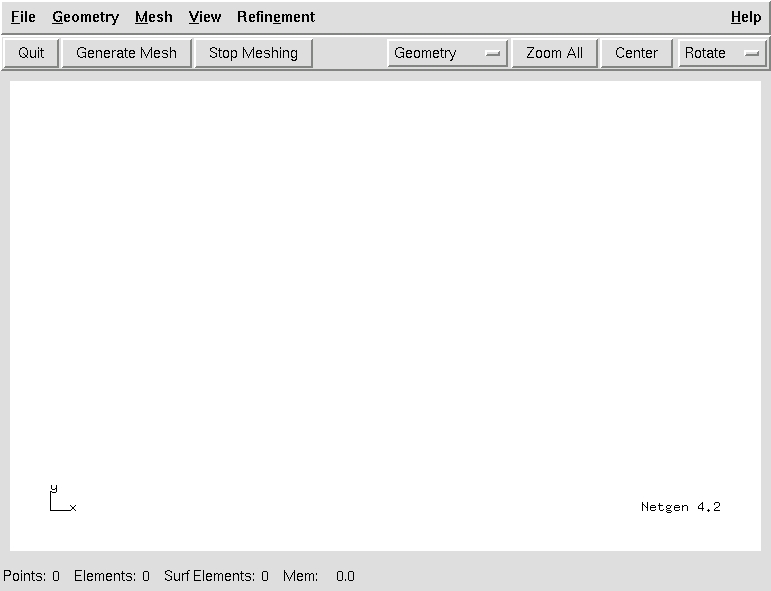
\includegraphics[width=12cm]{pictures/screenshot}
\end{center}
It consists of the menuline and the button line at the top, the status line at
the bottom, and the large drawing window. The menu items will be explained in 
\ref{sec_menuitems}. The button line provides shot-cuts for common opteration:
\begin{itemize}
\item Quit \newline
Terminate Netgen
\item Generate mesh \newline
Perform mesh generation 
\item Stop Meshing \newline
Stop mesh generation 
\item Geometry/Edges/Mesh/Solution \newline
Switch between operation modes of visualization.
\item Zoom all \newline
Zooms such that the whole visualization scene fits into the window.
\item Center \newline
Center rotation and scaling at marked point, available only in mesh - visuailzation mode.
\item Rotate/Move/Zoom
Left mouse drag rotates/moves/zooms object.
\end{itemize}

The status line shows information, namely
\begin{itemize}
\item Points \newline
Number of points in the mesh
\item Elements \newline
Number of volume elements (3D) in the mesh
\item Surf Elements \newline
Number of surface elements (3D) or inner elements (2d) in the mesh.
\item Mem \newline
Used memory in the large memory arena
\item Meshing Job, percentage
Douriing mesh generation, the current job as well as the progress is displayed on the 
right side of the statu line.
\end{itemize}

The drawing window displays the geometry or the mesh. The view
can be changed with the mouse:
\begin{itemize}
\item drag with left button pressed rotates the object,
\item drag with middle button pressed moves the object,
\item drag with right button pressed zooms the object.
\end{itemize}
The view can also be changed with the keyboard:
\begin{itemize}
\item cursor keys rotate the object
\item shift + cursor keys move the object
\item control + cursor keys zoom the object
\end{itemize}

When in Mesh - visualization scene, double clicking on triangles mark the
surface. The point cursor is set.

\section{The Netgen menu items}
\label{sec_menuitems}
\subsection{The menu item {\em File}}
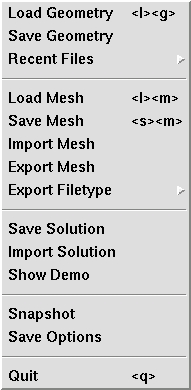
\includegraphics[height=7.8cm]{pictures/menufile} 

\subsection{The menu item {\em Geometry}}
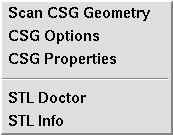
\includegraphics[height=2.7cm]{pictures/menugeometry} 

\subsection{The menu item {\em Mesh}}
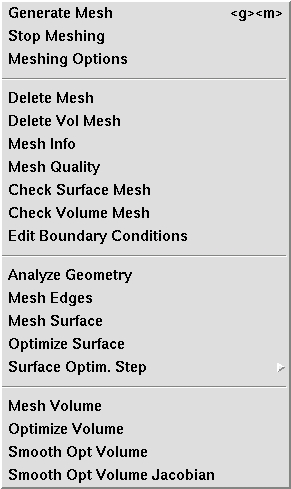
\includegraphics[height=9.8cm]{pictures/menumesh} 

\subsection{The menu item {\em View}}
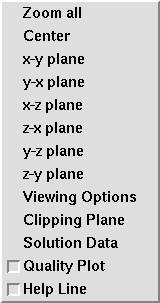
\includegraphics[height=6.0cm]{pictures/menuview} 

\subsection{The menu item {\em Refinement}}
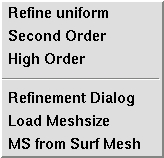
\includegraphics[width=3.2cm]{pictures/menurefinement} 


\section{Meshing Options}

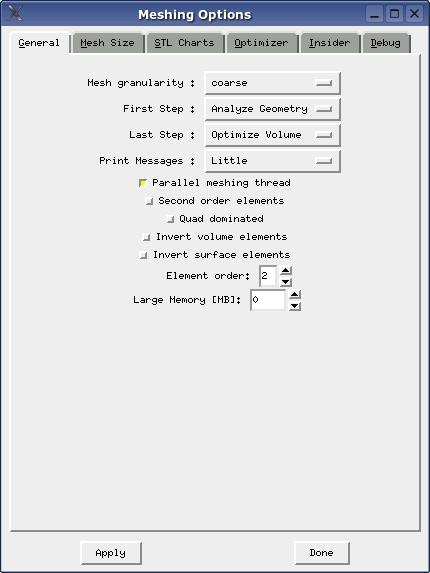
\includegraphics[width=10cm]{pictures/meshingoptions_1} 

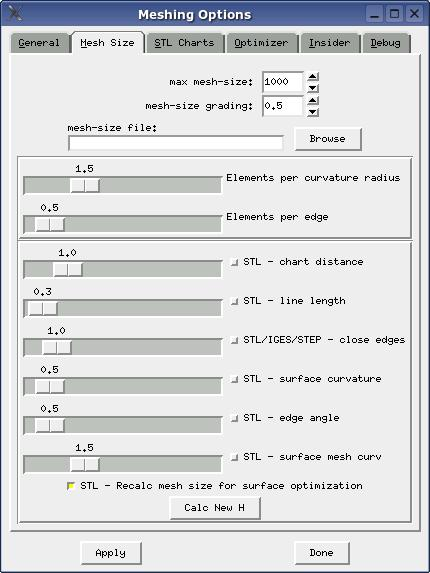
\includegraphics[width=10cm]{pictures/meshingoptions_2} 

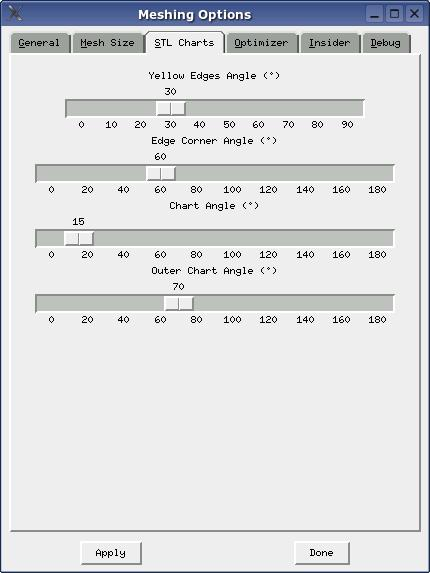
\includegraphics[width=10cm]{pictures/meshingoptions_3} 

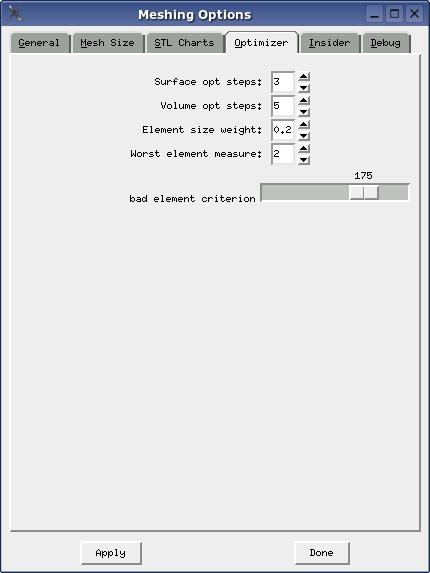
\includegraphics[width=10cm]{pictures/meshingoptions_4} 

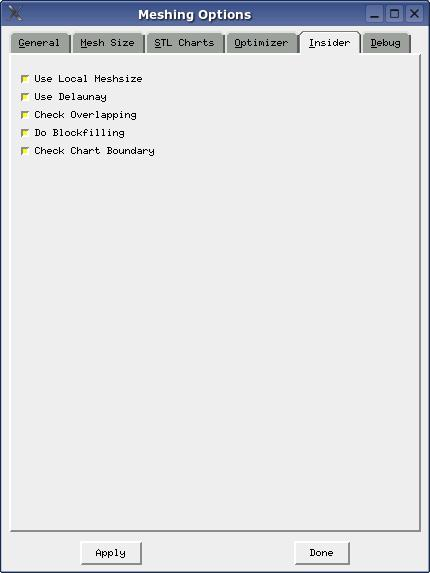
\includegraphics[width=10cm]{pictures/meshingoptions_5} 

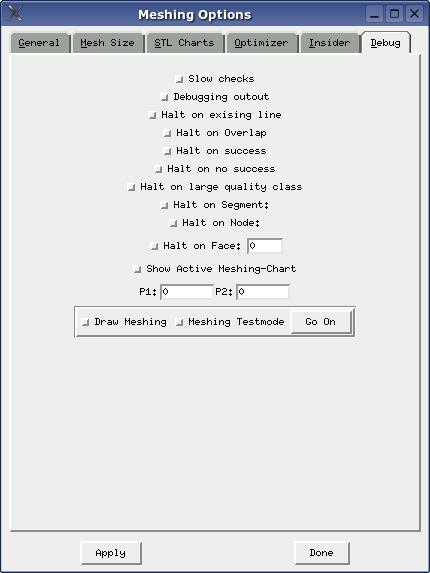
\includegraphics[width=10cm]{pictures/meshingoptions_6} 


\section{Visualization Options}



% \chapter{The Algorithms of Netgen}
%
% Netgen follows a top down strategy. It starts from computing the
% corner points (CSG only). Then, the edges are defined and meshed into
% segments (CSG and STL). Next, the faces are meshed by an advancing front
% surface mesh generator. After meshing, the faces meshes are optimized.
% Finally, the individual sub-domains are filled with tets. Therefore, 
% a fast Delaunay algorithm generates most of the elements (about 98 percent).
% But often it fails for mesh the whole domain, then the slower back-tracking
% rule-base algorithm takes over. Finally, the volume is optimized by the
% usual node - movement, element swapping and splitting algorithms.


\chapter{Programming Interfaces}
%
\section{The nginterface}
By means of the nginterface one's own simulation code can be 
included into the netgen environment. This is particular useful
for FEM (FVM,BEM) code developers, since they may profit from the
netgen preprocessing and postprocessing possibilities. 

Please download the example Netgen-add-on module {\it demoapp} and
follow the instructions therein

\section{The nglib}


\subsection{Introduction}
The NETGEN mesh generation library {\it nglib} is available in C++
source code and can be compiled for Unix/Linux as well as Win95/98/NT
and linked to one library file. The interface to the application
programme is by the C language header file {\it nglib.h}.

The functionality of nglib is volume mesh generation by a domain given 
by a surface triangulation, and surface mesh generation from a domain 
described by an STL file (standard file format for geometries defined by
triangle approximation). It can do mesh optimization as well as mesh 
refinement. It can generate 4 node tetrahedra and 10 node tetrahedrons
(with quadratic shape functions). The local mesh size can be defined 
automatically by geometric features and/or by user specification.


\subsection{The Header File}

The interface file contains the following type definitions and function
calls. All Netgen types and functions start with {\tt Ng}. Types and
functions have capital initial letters, constants are in capital letters.

\subsection{Types and Constants}
\begin{verbatim}

/// Data type for NETGEN mesh
typedef void * Ng_Mesh;

/// Data type for NETGEN STL geomty
typedef void * Ng_STL_Geometry;


// max number of nodes per element
#define NG_VOLUME_ELEMENT_MAXPOINTS 10

// implemented element types:
enum Ng_Volume_Element_Type { NG_TET = 1, NG_PYRAMID = 2, NG_PRISM = 3,
                              NG_TET10 = 4 };

// max number of nodes per surface element
#define NG_SURFACE_ELEMENT_MAXPOINTS 6

// implemented element types:
enum Ng_Surface_Element_Type { NG_TRIG = 1, NG_QUAD = 2, 
                                NG_TRIG6 = 3 };


struct Ng_Meshing_Parameters 
{
  double maxh;
  double fineness;   // 0 .. coarse, 1 .. fine
  int secondorder;
};

enum Ng_Result { NG_OK = 0, 
                 NG_SURFACE_INPUT_ERROR = 1,
                 NG_VOLUME_FAILURE = 2, 
                 NG_STL_INPUT_ERROR = 3,
                 NG_SURFACE_FAILURE = 4 };
\end{verbatim}


{\tt Ng\_Mesh} is a data type representing a Netgen mesh. {\tt Ng\_STL\_Geometry}
represents an STL geometry. One can operate on these data structures by
the functions defined below. Netgen can (now and/or in future) work with
various element types defined by generic constants. Several parameters
can be specified in the {\tt Ng\_Meshing\_Parameters} structure for 
volume and/or surface mesh generation. The result of Netgen functions
is of type {\tt Ng\_Result}.



\subsection{Initialization}
Please call these functions before using netgen functions and after
using netgen functions, respectively:
\begin{verbatim}
  // initialize, deconstruct Netgen library:
  void Ng_Init ();
  void Ng_Exit ();
\end{verbatim}


\subsection{Mesh access}
Netgen meshes can be processed by the means of the following functions.
A mesh contains nodes, surface elements and volume elements. Counting
starts from 1.

\begin{verbatim}
  // Generates new mesh structure
  Ng_Mesh * Ng_NewMesh ();
  void Ng_DeleteMesh (Ng_Mesh * mesh);
  
  // feeds points, surface elements and volume elements to the mesh
  void Ng_AddPoint (Ng_Mesh * mesh, double * x);
  void Ng_AddSurfaceElement (Ng_Mesh * mesh, Ng_Surface_Element_Type et,
                             int * pi);
  void Ng_AddVolumeElement (Ng_Mesh * mesh, Ng_Volume_Element_Type et,
                            int * pi);
  
  // ask for number of points, surface and volume elements
  int Ng_GetNP (Ng_Mesh * mesh);
  int Ng_GetNSE (Ng_Mesh * mesh);
  int Ng_GetNE (Ng_Mesh * mesh);

  
  //  return point coordinates
  void Ng_GetPoint (Ng_Mesh * mesh, int num, double * x);

  // return surface and volume element in pi
  Ng_Surface_Element_Type 
  Ng_GetSurfaceElement (Ng_Mesh * mesh, int num, int * pi);

  Ng_Volume_Element_Type
  Ng_GetVolumeElement (Ng_Mesh * mesh, int num, int * pi);
\end{verbatim}


\subsubsection{Mesh Generation}
The user can specify the mesh size function by the global parameter
maximal mesh size, and can additionally restrict the mesh size in
points or cubes. The function {\tt Ng\_GenerateVolumeMesh} generates
the volume mesh starting from the surface.

\begin{verbatim}
  // Defines MeshSize Functions
  void Ng_RestrictMeshSizeGlobal (Ng_Mesh * mesh, double h);
  void Ng_RestrictMeshSizePoint (Ng_Mesh * mesh, double * p, double h);
  void Ng_RestrictMeshSizeBox (Ng_Mesh * mesh, double * pmin, double * pmax, double h);
  
  // generates volume mesh from surface mesh
  Ng_Result Ng_GenerateVolumeMesh (Ng_Mesh * mesh, Ng_Meshing_Parameters * mp);
\end{verbatim}


\subsection{STL Geometry}
A STL geometry can be read from a STL file (ASCII or binary), or can
be assembled by providing triangle by triangle. Either, the user
can specify the edges of the geometry, or netgen can define edges 
by {\tt Ng\_STL\_MakeEdges} by using an angle criterium.

\begin{verbatim}
  // loads geometry from STL file
  Ng_STL_Geometry * Ng_STL_LoadGeometry (char * filename, int binary = 0);

  // generate new STL Geometry
  Ng_STL_Geometry * Ng_STL_NewGeometry ();
  
  // fills STL Geometry
  // positive orientation
  // normal vector may be null-pointer
  void Ng_STL_AddTriangle (Ng_STL_Geometry * geom, 
                           double * p1, double * p2, double * p3, double * nv);

  // add (optional) edges:
  void Ng_STL_AddEdge (Ng_STL_Geometry * geom, 
                       double * p1, double * p2);


  // after adding triangles (and edges) initialize
  Ng_Result Ng_STL_InitSTLGeometry (Ng_STL_Geometry * geom);

  // automatically generates edges:
  void Ng_STL_MakeEdges (Ng_STL_Geometry * geom);

    // generates mesh, empty mesh be already created.
  Ng_Result Ng_STL_GenerateSurfaceMesh (Ng_STL_Geometry * geom,
                                        Ng_Mesh * mesh,
                                        Ng_Meshing_Parameters * mp);
\end{verbatim}

\subsection{Programming Example}

The File {\it ngcore.cc}, see Appendix A, is a simple application
using the netgen volume mesh generator. First, the surface mesh
is read from a file containing point coordinates and surface triangles
(see e.g. file {\it cube.surf}). The volume mesh generate is called, 
and the volume mesh is written to the standard output, see file {\it cube.vol}.



\end{document}
